\subsection{Beyond P}
We have painted a rosy picture for algorithmic solutions, by picking problems that have polynomial time solutions and designing poly-time algorithm for them. However, the problems you will encounter in the real world and in your careers will not have such efficient solutions. 

Many of these decision problems share an interesting feature: if you are given a YES instance of the problem, and a ``solution'' to this YES instance, then you can verify that this is a YES instance in polynomial time.

For example,
\begin{itemize}
	\item A Hamilton Cycle (HC) in a graph is a simple cycle that passes through all vertices without hitting any vertex twice.
	\item The HC decision problem is: given a graph $G$, does it have a Hamilton Cycle?
	\item We believe it is a hard problem, but if a certain $G$ is a YES instance, and we were also given the Hamilton cycle itself, we could efficiently verify this and confirm that it is a YES instance.
\end{itemize}

The verification algorithm is given two inputs: $G$ and a proposed Hamilton cycle $v_1, v_2, \cdots, v_n, v_1$.
\begin{itemize}
	\item It first checks that the cycle is simple and passes through all vertices, by checking that every vertex occurs and that no vertex occurs twice (expect the start and end vertices).
	\item Next, it confirms that each $(v_i, v_{i+1})$ for $i = 1, 2, \cdots, n-1$ is an edge in $G$. It also checks that $(v_n, v_1)$ is an edge.
	\item Now it is convinced that $G$ is a YES instance.
\end{itemize}
Note that we are not saying that we can efficiently find the Hamilton Cycle! We are just saying that, given the cycle, we can verify that $G$ is a YES instance.

\subsection{``NP''}
Many difficult problems you will encounter share this property: for YES instance, there is a ``solution'' that can be easily verified. Such a solution is called many names: certificate, proof, or witness.

A decision problem $\pi$ is in \textbf{NP} (read as ``non-deterministic polynomial time'') if there is a polynomial time verification algorithm $V$ such that:
\begin{itemize}
	\item If $x$ if a YES instance of $\pi$, there exists a certificate $y$ whose length is polynomial in $|x|$ such that $V(x, y)$ accepts.
	\item If $x$ is a NO instance of $\pi$, then for any string $y$, $V(x, y)$ rejects.
\end{itemize}

Again, note that we are not talking about computing $y$ efficiently. In fact, we believe that, for many problems in \textbf{NP}, there is no efficient way to compute $y$.
\subsection{Examples}
\subsubsection{Maximum Clique Problem}
Given a graph $G$ and a number $K$, are there $K$ vertices in $G$ that are all pairwise adjacent? Such group of vertices are called clique.

This kind of problem is useful for finding groups of mutual friends in social networks.

Certificate: the $K$ vertices that form the clique. Verification is straightforward.

\begin{figure}[H]
	\centering
	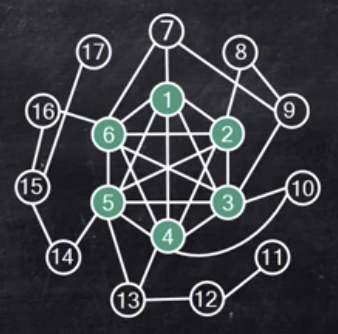
\includegraphics[width=0.3\textwidth]{fig/max-clique-2.png}
\end{figure}

\subsubsection{3-Coloring Problem}
Given a graph $G$, can we assign 3 colors to its vertices so that any pair of adjacent vertices have different colors?

This kind of problem is useful for allocating frequencies to radio stations to avoid interference, deciding which activities to schedule in which rooms, or allocating registers to variables in a program.

Certificate: the colors of the vertices. Easy to verify coloring by examining all edges.

\begin{figure}[H]
	\centering
	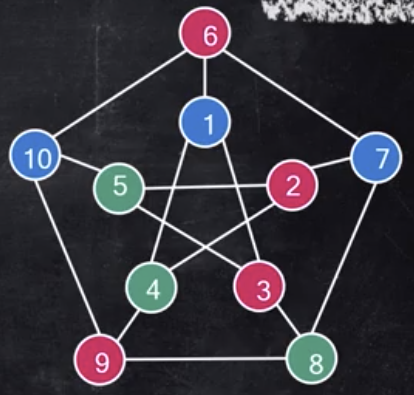
\includegraphics[width=0.3\textwidth]{fig/3-color.png}
\end{figure}

\subsubsection{Partition Problem}
Given $n$ numbers, can they be partitioned into 2 sets such that the sums of the numbers in the sets are equal?

Certificate: the actual partition into two sets. Easy to verify that each part adds to the same total.

\begin{figure}[H]
	\centering
	
\includegraphics[width=0.3\textwidth]{fig/partition.png}
\end{figure}

\subsection{Asymetry In Definitions of P and NP}
For a problem $\pi$ to be in NP, only the YES instances have certificates accepted by the verifier. There aren't any certificates for the NO instance. So if you are given an instance of the clique problem $(G, K)$, we do not know any short certificate that will demonstrate that $G$ does not have a clique of size $K$.

Example: an integer $N$ is composite if it has a factor $p$: $1 < p < N$.
\begin{itemize}
	\item Composites are in NP.
	\item Given a YES instance i.e. a composite number, a certificate demonstrating that $N$ is composite is a non-trivial factor $p$.
	\item It is not immediately clear that NO instance are also efficiently verifiable.
	\item Given $N$ that is not a composite, i.e. a prime number, what would a certificate be?
	\item In this case, it turns out that there are certificates for primality but understanding how they work requires some knowledge of abstract algebra.
\end{itemize}

\subsection{``Co-NP''}
Given the asymmetry we observed, we could define a complexity class of problems for which NO instances can be efficiently verified. This is the class \textbf{Co-NP}.

The complement of a decision problem $\pi$ is the problem $\pi'$ defined as: $x$ is a YES instance of $\pi$ if and only if it is a NO instance of $\pi'$.

A problem $\pi'$ is in Co-NP if and only if its complement $\pi$ is in NP.


\subsection{Turing Machine Definition of NP}
A problem is in NP if there exists a non-deterministic TM that can decide if $x$ is a YES or NO instance in polynomial time.













